\section{$\text{LTL}_f/\text{LDL}_f$ Non-Markovian Rewards}
Recently, non-Markovian reward decision processes (NMRDPs)
has attracted interest in the scientific community because of the possibility
of specifying them as MDPs with $\text{LTL}_f/\text{LDL}_f$ non-Markovian
rewards \cite{DBLP:journals/corr/abs-1807-06333}. In particular, it is possible
to model the problem with two separate representations of the world, one for
the agent (low-level) and one for the goal (expressed in terms of high-level
fluents).

This section presents the approach used in
\cite{DBLP:journals/corr/abs-1807-06333}, where an efficient method has been
developed in order to work with NMRDPs. The theory behind the main idea is
quickly described and an example on a theoretical Breakout environment is
discussed in order to be used in the following sections easily.

\subsection{Theoretical Background}
Before describing the problem, let's give a formal definition of NMRDP.
A non-Markovian reward decision process is a tuple $M = \langle S, A, \delta,
\bar{R} \rangle$, with $S$ finite set of states that can represent the
environment, $A$ is a finite set of actions that can be performed by an agent
in the environment, $\delta$ is a probability function modeling
the transition from a state to another when performing a certain action and
$\bar{R}: (S \times A)^* \rightarrow \mathbb{R}$ is a function from
finite state-action sequences (traces) to real-values that represents the
reward given by the environment when performing a certain state-action
sequence. Specifying a non-Markovian reward function explicitely is
difficult even when considering a finite number of traces. Luckily, the
$\text{LTL}_f/\text{LDL}_f$ formalism allows to specify $\bar{R}$
implicitely using a set of pairs $\{ (\phi_i, r_i) \}_{i=1}^m$ with
$\phi_i$ boolean
proposition over the components of the state vector and $r_i$ such that,
given a current trace $\pi = \langle s_, a_1, \dots, s_{n-1}, a_n \rangle$,
the agent receives at $s_n$ a reward $r_i$ if $\phi_i$ is satisfied by $\pi$,
hence:
\begin{equation}
    \bar{R}(\pi) =
        \begin{cases}
            r_i & \text{if } \pi \vDash \phi_i \\
            0 & \text{otherwise}
        \end{cases}
\end{equation}

Since the NMRDP rewards are based on traces, instead of state-action pairs,
typical learning algorithms like Q-learning or SARSA cannot be used.
Nevertheless, it has been shown \cite{DBLP:journals/corr/abs-1807-06333} that
for any NMRDP $M = \langle S, A, \delta, \{ (\phi_i, r_i) \}_{i=1}^m \rangle$
there exists an MDP $M' = \langle S', A', \delta' R' \rangle$ that is equivalent
to $M$. The idea behind the proof consists in starting from an initial
decision process $M_{ag}^{goal} = \langle S, A, R, \mathcal{L},
\delta_{ag}^g, \{ (\phi_i, r_i) \}_{i=1}^m \rangle$ with
$\text{LTL}_f/\text{LDL}_f$ goals (with $\mathcal{L}$ set of of configuration
of the high-level features needed for expressing $\phi_i$),
transform it into a NMRDP in order to
further transform it into a MDP where it is possible to execute learning
algorithms such as Q-learning. All the details are out of the scope of the
project and are discussed in \cite{DBLP:journals/corr/abs-1807-06333}. The
set of states $S$ is used to express low-level features of the agent.
\begin{figure}
    \centering
    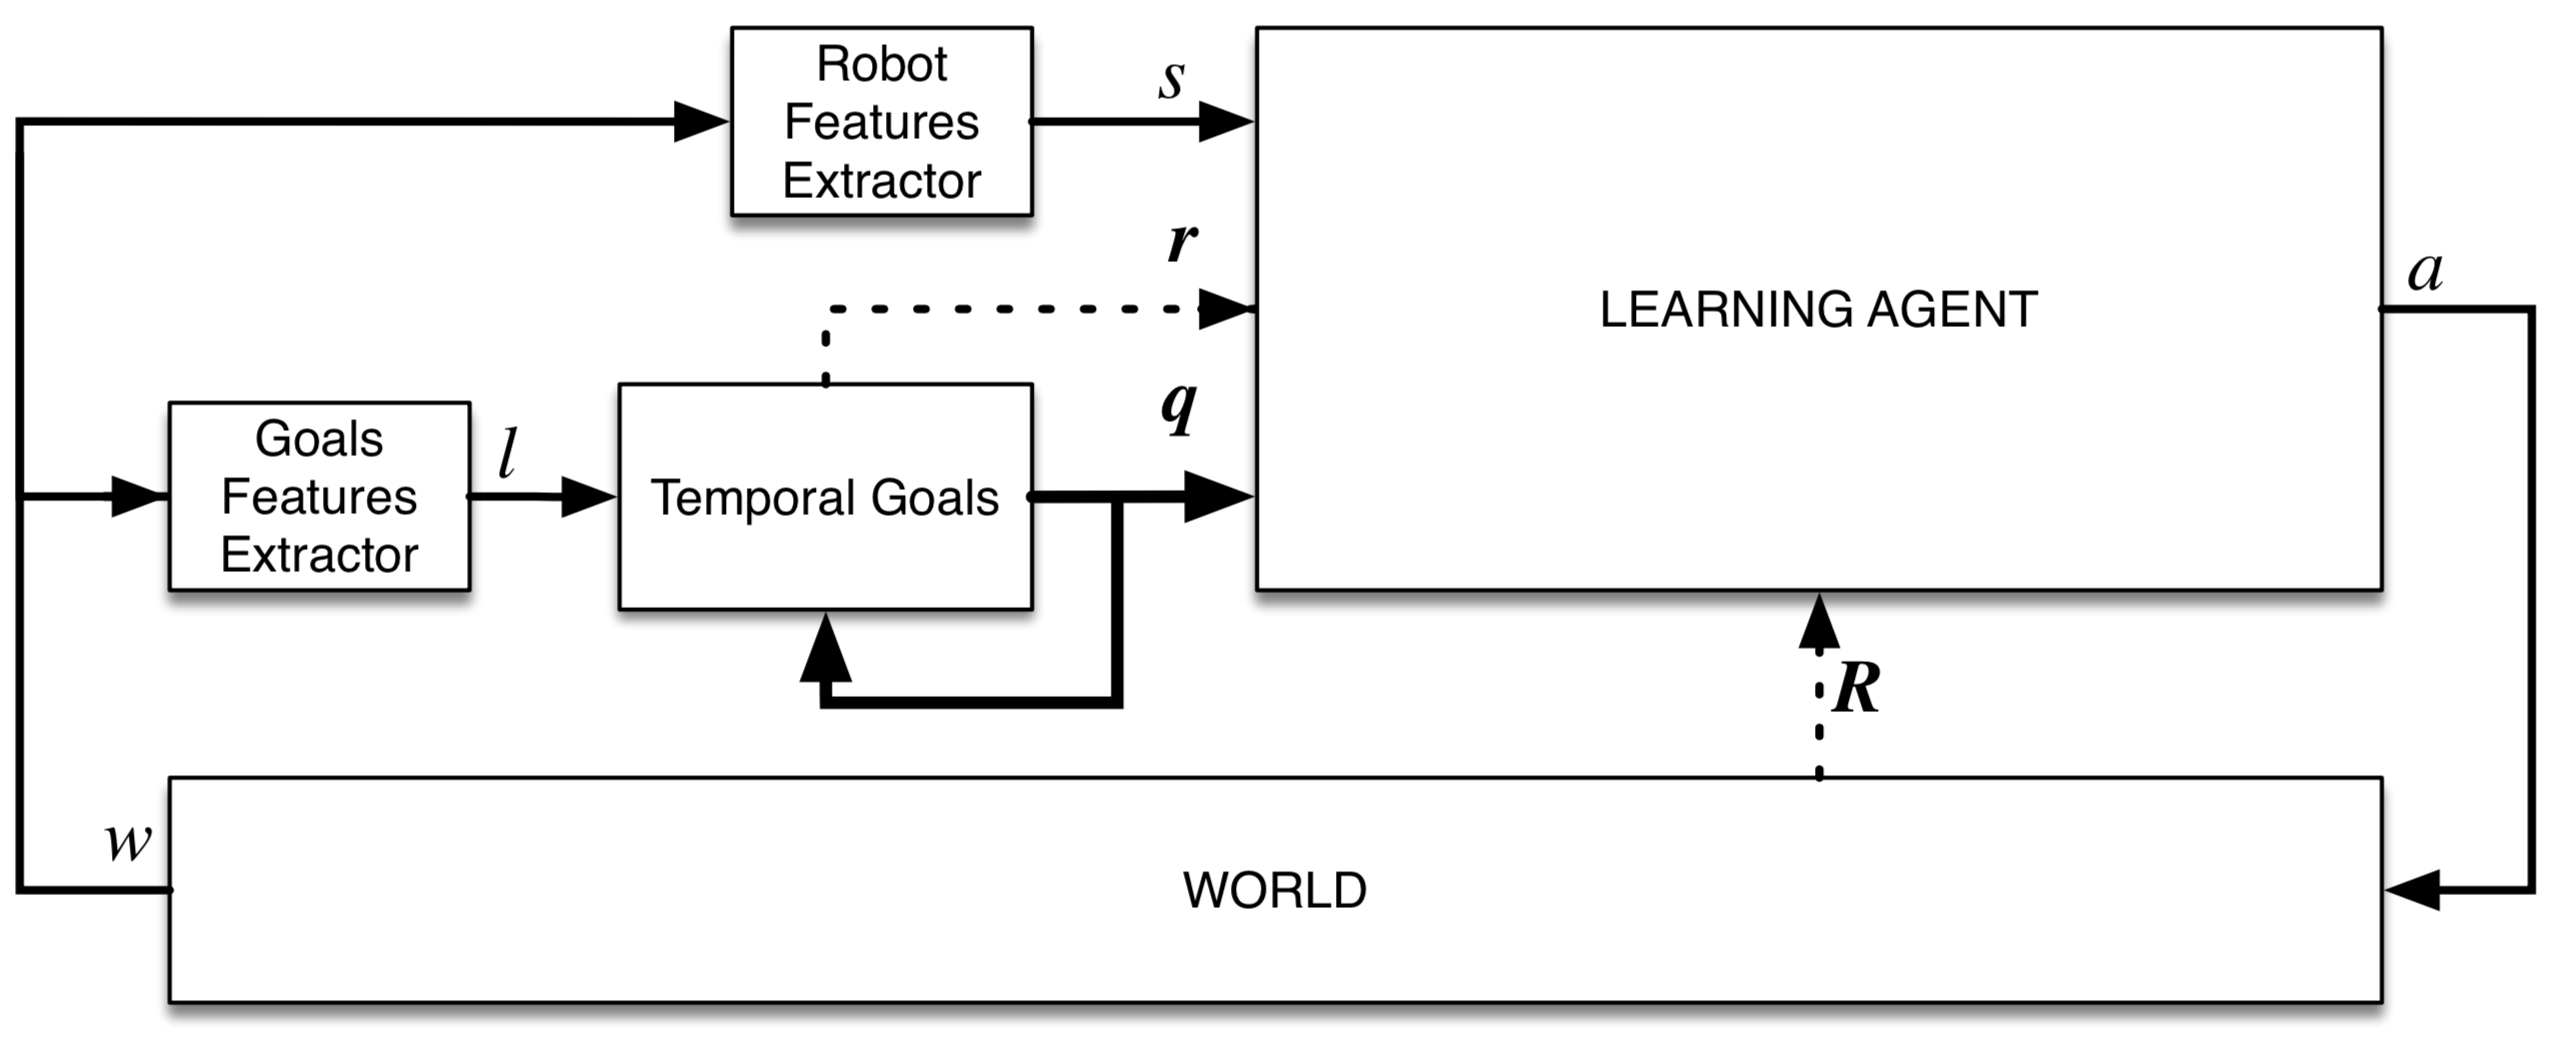
\includegraphics[width=0.85\textwidth]{images/rl-temporalgoals-pipeline.png}
    \caption{TODO: description.}
    \label{fig:rl-temporalgoals-pipeline}
\end{figure}

\subsection{Examples}
How it can be used to train a RL model.
